% =====================================================================
%  Processamento de Imagens - Avaliacao Bimestral (1o Bimestre)
%  Sistema de Analise Automatica de Objetos em uma Imagem
%
%  Compilar com:  pdflatex relatorio.tex   (duas vezes, pelo sumario)
% =====================================================================
\documentclass[12pt,a4paper]{article}

\usepackage[utf8]{inputenc}
\usepackage[T1]{fontenc}
\usepackage[brazil]{babel}
\usepackage[margin=2.5cm]{geometry}
\usepackage{graphicx}
\usepackage{booktabs}
\usepackage{caption}
\usepackage{subcaption}
\usepackage{float}
\usepackage{amsmath}
\usepackage{listings}
\usepackage{xcolor}
\usepackage[hidelinks]{hyperref}

\graphicspath{{imagens/}}

\lstset{
  basicstyle=\ttfamily\footnotesize,
  language=C++,
  keywordstyle=\color{blue!60!black},
  commentstyle=\color{green!40!black}\itshape,
  numbers=left, numberstyle=\tiny\color{gray},
  frame=single, framesep=4pt, breaklines=true,
  showstringspaces=false, tabsize=4,
}

\title{\textbf{Sistema de Análise Automática de Objetos em uma Imagem}}
\author{%
  % >>> PREENCHER com os nomes da equipe (até 3 alunos) <<<
  Nome do aluno 1 \\
  Nome do aluno 2 \\
  Nome do aluno 3
}
\date{Ciência da Computação --- Universidade Tuiuti do Paraná \\[2pt]
      Processamento de Imagens --- Prof.\ Diógenes Furlan \\[2pt]
      Avaliação Bimestral --- 1\textsuperscript{o} Bimestre --- 2026}

\begin{document}

\maketitle
\thispagestyle{empty}

\begin{abstract}
\noindent
Este trabalho apresenta um sistema capaz de analisar automaticamente uma
imagem digital contendo um ou mais objetos, separando-os do fundo,
identificando cada um individualmente e calculando suas características
geométricas. O sistema foi implementado em C++ com OpenGL/GLUT e encadeia
técnicas básicas de processamento digital de imagens: conversão para tons de
cinza, filtragem espacial, análise de histograma, limiarização automática por
Otsu, morfologia matemática e rotulação de componentes conexos. Para cada
objeto identificado são calculadas área, centroide, \emph{bounding box},
perímetro e circularidade. O sistema foi testado em três imagens de
dificuldade crescente e identificou corretamente todos os objetos nas três.
\end{abstract}

\tableofcontents
\newpage

% =====================================================================
\section{Introdução}
% =====================================================================

O problema tratado neste trabalho é o da \textbf{análise automática de
objetos} em uma imagem digital. Dada uma imagem contendo um ou mais objetos
sobre um fundo contrastante, o sistema deve determinar, sem intervenção do
usuário, quantos objetos existem, onde cada um está e quais são suas
características geométricas.

As imagens trabalhadas são arquivos BMP de 8 e 24 bits, convertidos
internamente para tons de cinza. Três situações foram consideradas, conforme
pedido no enunciado:

\begin{enumerate}
  \item \textbf{Situação simples}: objetos bem separados e com alto contraste
        em relação ao fundo;
  \item \textbf{Presença de ruído}: a mesma imagem contaminada com ruído
        sal-e-pimenta, exigindo pré-processamento;
  \item \textbf{Situação mais complexa}: objetos de tamanhos e formas
        diferentes, incluindo figuras vazadas (apenas o contorno).
\end{enumerate}

O objetivo do trabalho é integrar as técnicas estudadas ao longo do bimestre,
mostrando como algoritmos individualmente simples --- uma contagem de pixels,
uma comparação com um limiar, uma varredura de vizinhança --- se combinam
para resolver um problema de análise que nenhum deles resolveria sozinho.

Um objetivo secundário, que orientou várias decisões de projeto, foi tornar
cada etapa \textbf{observável}: o programa permite executar o pipeline passo a
passo, exibindo o resultado intermediário de cada operação, de modo que o
efeito de cada técnica sobre a imagem possa ser visto e discutido
isoladamente.

% =====================================================================
\section{Fundamentação Teórica}
% =====================================================================

\subsection{Histograma}

O histograma de uma imagem em tons de cinza é a contagem de quantos pixels
existem para cada nível de intensidade. Para uma imagem de 8 bits, é um vetor
de 256 posições em que $h[k]$ guarda o número de pixels com intensidade $k$:

\begin{equation}
h[k] = \#\{(x,y) \mid f(x,y) = k\}, \qquad k = 0,1,\dots,255
\end{equation}

A soma de todas as posições é necessariamente o número total de pixels,
$\sum_{k=0}^{255} h[k] = L \times C$. O histograma normalizado, obtido
dividindo-se cada posição por $L \times C$, estima a probabilidade de um pixel
qualquer ter determinada intensidade.

A distinção fundamental é que a \textbf{imagem} carrega informação espacial
enquanto o \textbf{histograma} carrega informação estatística: a posição dos
pixels é descartada. Duas imagens completamente diferentes podem ter
histogramas idênticos. É justamente por ser estatístico que ele serve para
escolher um limiar sem precisar saber onde os objetos estão.

\subsection{Filtragem espacial}

Filtros espaciais combinam a intensidade de um conjunto de pixels vizinhos
para gerar a intensidade do pixel correspondente na imagem de saída. Foram
implementados dois, com propósitos distintos.

\paragraph{Filtro de média.} É um filtro passa-baixa, obtido pela convolução
com uma máscara cujos coeficientes são positivos e somam~1:

\begin{equation}
w = \frac{1}{9}
\begin{bmatrix}
1 & 1 & 1 \\
1 & 1 & 1 \\
1 & 1 & 1
\end{bmatrix}
\qquad
g(x,y) = \sum_{i}\sum_{j} w(i,j)\, f(x+i,\, y+j)
\end{equation}

Atenua as altas frequências --- as transições abruptas --- reduzindo ruído,
mas borrando as bordas junto.

\paragraph{Filtro de mediana.} Substitui cada pixel pela mediana das
intensidades da vizinhança, isto é, pelo valor central da lista ordenada dos
nove valores. É um filtro \textbf{não linear}: não há convolução de máscara,
porque ordenar não é uma operação linear e nenhum conjunto de coeficientes o
reproduz.

A vantagem sobre a média aparece no ruído impulsivo. Um pixel de valor extremo
(0 ou 255) isolado em uma vizinhança homogênea vai parar em uma das pontas da
lista ordenada e é simplesmente descartado, em vez de ser diluído na soma e
contaminar o resultado --- e, com ele, o dos oito vizinhos.

\subsection{Limiarização}

A limiarização converte a imagem de 256 níveis em uma imagem binária,
comparando cada pixel com um valor de corte~$T$:

\begin{equation}
b(x,y) =
\begin{cases}
1 & \text{se } f(x,y) > T \quad \text{(objeto)} \\
0 & \text{caso contrário} \quad\;\; \text{(fundo)}
\end{cases}
\end{equation}

É a operação que cria a marcação sobre a qual todas as etapas seguintes
operam: morfologia, rotulação e medidas geométricas só existem sobre imagem
binária.

\paragraph{Método de Otsu.} Escolher $T$ manualmente não é aceitável em um
sistema automático. O método de Otsu percorre todos os 256 cortes possíveis e
escolhe o que \textbf{maximiza a variância entre as duas classes}, o que é
equivalente a minimizar a variância dentro de cada classe:

\begin{equation}
\sigma_b^2(T) = \omega_0(T)\,\omega_1(T)\,\big[\mu_0(T) - \mu_1(T)\big]^2
\end{equation}

\noindent onde $\omega_0$ e $\omega_1$ são as quantidades de pixels de cada
classe e $\mu_0$ e $\mu_1$ suas intensidades médias. Intuitivamente: procura o
corte que deixa os dois grupos mais separados entre si e mais homogêneos
internamente. O cálculo usa apenas o histograma, sem varrer a imagem
novamente.

\subsection{Morfologia matemática}

A morfologia matemática extrai informação sobre a geometria de um conjunto
desconhecido transformando-o por meio de outro conjunto bem definido, o
\textbf{elemento estruturante}. Neste trabalho o elemento estruturante é
$3\times3$ preenchido, correspondente à vizinhança-8.

\paragraph{Erosão.} $A \ominus B$ --- o pixel permanece objeto apenas se
\emph{todos} os pixels sob o elemento estruturante forem objeto. É a operação
\textsc{and} da vizinhança. Contrai os objetos em uma camada, eliminando
pontos isolados e saliências finas.

\paragraph{Dilatação.} $A \oplus B$ --- o pixel vira objeto se \emph{algum}
pixel sob o elemento estruturante for objeto. É a operação \textsc{or}.
Expande os objetos em uma camada, preenchendo buracos pequenos.

As duas são duais: o complemento de uma erosão é a dilatação do complemento
pelo elemento estruturante refletido, $(A \ominus B)^c = A^c \oplus \hat{B}$.

\paragraph{Abertura e fechamento.} São as composições das duas primitivas:

\begin{align}
A \circ B &= (A \ominus B) \oplus B \qquad \text{(abertura)} \\
A \bullet B &= (A \oplus B) \ominus B \qquad \text{(fechamento)}
\end{align}

Na abertura, a erosão apaga o ruído e a dilatação seguinte devolve aos objetos
sobreviventes o tamanho original --- limpa sem encolher. No fechamento, a
dilatação tapa buracos e fendas e a erosão recupera o contorno externo. A
ordem importa: as duas operações não são comutativas, e cada uma resolve um
problema para o qual a outra é cega.

\subsection{Componentes conexos}

Dois pixels $p$ e $q$ pertencentes ao conjunto $S$ são conexos se existe um
caminho entre eles formado inteiramente por pixels de $S$. O conjunto de todos
os pixels conexos a um dado pixel é um \textbf{componente conexo}. Rotular os
componentes é o que permite contar objetos e tratá-los individualmente.

A definição depende da relação de adjacência adotada:

\begin{itemize}
  \item \textbf{Adjacência-4}: vizinhos horizontais e verticais,
        $N_4(p) = \{(x{\pm}1,y),\,(x,y{\pm}1)\}$;
  \item \textbf{Adjacência-8}: os quatro anteriores mais os quatro diagonais,
        $N_8(p) = N_4(p) \cup N_D(p)$.
\end{itemize}

A escolha altera o resultado: uma mesma figura pode apresentar 4 regiões por
adjacência-8 e 10 por adjacência-4, porque nesta última objetos ligados apenas
pela diagonal são contados separadamente. Este trabalho usa
\textbf{adjacência-8}, que corresponde melhor à noção intuitiva de objeto.

\subsection{Características geométricas}

Para cada componente rotulado com o identificador $r$, sendo
$R = \{(x,y) \mid \text{rótulo}(x,y) = r\}$:

\begin{description}
  \item[Área] $A = |R|$, o número de pixels do objeto.

  \item[Centroide] as coordenadas médias dos pixels do objeto:
    \begin{equation}
      \bar{x} = \frac{1}{A}\sum_{(x,y) \in R} x
      \qquad
      \bar{y} = \frac{1}{A}\sum_{(x,y) \in R} y
    \end{equation}

  \item[\emph{Bounding box}] o menor retângulo que envolve o objeto,
    $(x_{\min}, y_{\min})$ a $(x_{\max}, y_{\max})$.

  \item[Perímetro] estimado pela contagem dos pixels de contorno, isto é,
    pixels do objeto que possuem ao menos um vizinho-4 fora dele.

  \item[Circularidade] razão adimensional que compara a área com o quadrado do
    perímetro:
    \begin{equation}
      C = \frac{4\pi A}{P^2}
      \label{eq:circ}
    \end{equation}
    Quanto mais compacta a forma, maior o valor. Serve para comparar formas
    entre si.
\end{description}

% =====================================================================
\section{Metodologia}
% =====================================================================

A sequência de processamento adotada é a seguinte:

\begin{center}
\framebox{\parbox{0.92\textwidth}{\centering
\textbf{leitura do BMP} $\rightarrow$ \textbf{conversão para tons de cinza}
$\rightarrow$ \textbf{filtro de mediana $3\times3$} $\rightarrow$
\textbf{histograma} $\rightarrow$ \textbf{limiarização por Otsu} $\rightarrow$
\textbf{abertura + fechamento} $\rightarrow$ \textbf{rotulação (8-conexa)}
$\rightarrow$ \textbf{filtro de área} $\rightarrow$
\textbf{análise geométrica}
}}
\end{center}

\medskip

A ordem difere do diagrama sugerido no enunciado em dois pontos, ambos
deliberados e justificados a seguir.

\paragraph{A morfologia vem antes da rotulação, não depois.} O diagrama do
enunciado posiciona os filtros morfológicos após a etapa de componentes
conexos. Optamos pela ordem inversa porque o propósito da morfologia neste
pipeline é \emph{limpar} a imagem binária, e limpá-la depois de contar os
objetos não altera a contagem já realizada --- que é o resultado que o
trabalho pede. Aplicada antes, a abertura elimina os pontos de ruído que de
outro modo seriam contados como objetos. A Seção~\ref{sec:discussao} apresenta
a medição que sustenta essa escolha.

\paragraph{O histograma é calculado antes da filtragem e novamente depois.}
O histograma tem dois papéis distintos: é instrumento de diagnóstico, usado
para entender a distribuição de intensidades da imagem e decidir se a
limiarização é viável, e é insumo do método de Otsu. No primeiro papel
interessa o histograma da imagem original; no segundo, o da imagem já
filtrada, que é sobre a qual o limiar será aplicado.

\paragraph{Filtro de área.} Após a rotulação, componentes com área inferior a
um limite (50 pixels, ajustável em tempo de execução) são descartados e os
rótulos restantes são renumerados. É a última barreira contra falsos objetos:
fragmentos de ruído que sobrevivem à filtragem e à morfologia são pequenos
demais para serem objetos reais.

\paragraph{Detecção automática de polaridade.} A limiarização precisa saber de
que lado do limiar estão os objetos, e isso varia conforme a imagem: em
\texttt{Circulos4.bmp} os objetos são claros sobre fundo escuro, e em
\texttt{C1.bmp} são escuros sobre fundo claro. O sistema decide sozinho
contando os pixels de cada lado do limiar e tomando como objeto a
\textbf{classe minoritária}, partindo do princípio --- declarado no enunciado
--- de que os objetos aparecem sobre um fundo contrastante e ocupam menos área
que ele. Sem esse mecanismo, metade das imagens de teste seria processada com
o fundo rotulado como um único objeto cobrindo a imagem inteira.

% =====================================================================
\section{Implementação}
% =====================================================================

O sistema foi escrito em C++ sobre o \emph{framework} fornecido na disciplina
(OpenGL com GLUT para exibição e uma biblioteca de leitura e escrita de BMP),
portado de Windows/Code::Blocks para Linux com \texttt{g++} e
\texttt{freeglut}. As alterações necessárias ao porte estão documentadas em
\texttt{codigo/PORTE.md}.

\subsection{Estrutura dos arquivos}

\begin{table}[H]
\centering
\begin{tabular}{ll}
\toprule
\textbf{Arquivo} & \textbf{Responsabilidade} \\
\midrule
\texttt{src/main.cpp}      & janela, teclado, menu e roteiros de demonstração \\
\texttt{src/pdi.cpp/.h}    & todos os algoritmos do pipeline \\
\texttt{src/image\_class.cpp/.h} & classe de imagem: pixels, exibição, arquivo \\
\texttt{src/bmp\_lib2.cpp/.h}    & leitura e escrita de arquivos BMP \\
\bottomrule
\end{tabular}
\caption{Organização do código-fonte.}
\end{table}

\subsection{Estruturas de dados}

A decisão de projeto mais importante foi não operar diretamente sobre os
pixels RGB da \texttt{ImageClass} a cada etapa. Em vez disso, a classe
\texttt{PDI} mantém buffers próprios, vetores planos de $W \times H$
posições, indexados sempre da mesma forma:

\begin{lstlisting}
int W, H;                      // dimensoes da imagem atual
vector<unsigned char> cinza;   // 0..255
vector<unsigned char> bin;     // 0 = fundo, 1 = objeto
vector<int> rotulo;            // 0 = fundo, 1..n = objetos
int histograma[256];
vector<Objeto> objetos;
\end{lstlisting}

O acesso é sempre \texttt{buf[y*W + x]}. A uniformidade elimina a principal
fonte de erro do trabalho --- confundir linha com coluna --- e mantém os dados
contíguos em memória.

As características de cada objeto são guardadas em um \texttt{struct}:

\begin{lstlisting}
struct Objeto {
    int id, area;
    double cx, cy;               // centroide
    int xmin, ymin, xmax, ymax;  // bounding box
    int perimetro;
    double circularidade;
};
\end{lstlisting}

\subsection{Principais funções}

\begin{table}[H]
\centering
\small
\begin{tabular}{ll}
\toprule
\textbf{Função} & \textbf{O que faz} \\
\midrule
\texttt{paraCinza()}            & converte a imagem de entrada para o buffer \texttt{cinza} \\
\texttt{calculaHistograma()}    & conta pixels por nível de intensidade \\
\texttt{filtroMedia3x3()}       & convolução com máscara de média \\
\texttt{filtroMediana3x3()}     & mediana da vizinhança $3\times3$ \\
\texttt{otsu()}                 & devolve o limiar ótimo a partir do histograma \\
\texttt{polaridadeAutomatica()} & decide de que lado do limiar está o objeto \\
\texttt{limiariza(T, claro)}    & preenche \texttt{bin} \\
\texttt{erosao()}, \texttt{dilatacao()} & primitivas morfológicas \\
\texttt{abertura()}, \texttt{fechamento()} & composições das primitivas \\
\texttt{rotulaComponentes()}    & rotula os componentes conexos; devolve a contagem \\
\texttt{floodFill()}            & preenchimento por inundação, 8-conexo \\
\texttt{analisaObjetos(areaMin)}& calcula as medidas e aplica o filtro de área \\
\texttt{imprimeRelatorio()}     & imprime a tabela no console \\
\texttt{desenhaObjetos()}       & imagem rotulada com cores, caixas e centroides \\
\texttt{pipelineCompleto()}     & encadeia tudo e grava as imagens intermediárias \\
\bottomrule
\end{tabular}
\caption{Principais funções da classe \texttt{PDI}.}
\end{table}

\subsection{Dois pontos de implementação que merecem destaque}

\paragraph{Filtros e morfologia leem de uma cópia.} Toda operação de
vizinhança lê de uma cópia do buffer e escreve no buffer original. Se lesse e
escrevesse no mesmo vetor, o pixel já processado contaminaria o cálculo do
vizinho seguinte, produzindo um arrasto direcional no resultado.

\paragraph{O \emph{flood fill} é iterativo, não recursivo.} A versão recursiva
apresentada em aula abre uma chamada de função por pixel visitado. Medimos
experimentalmente o limite: a versão recursiva sobrevive a um objeto de
$400\times400$ pixels, mas estoura a pilha em $512\times512$ --- exatamente o
tamanho do exemplo citado no enunciado. A implementação usa uma fila explícita
(\texttt{std::queue}), que aloca no \emph{heap} e não tem esse teto:

\begin{lstlisting}
void PDI::floodFill(int x0, int y0, int rot)
{
    queue< pair<int,int> > fila;
    rotulo[y0*W + x0] = rot;
    fila.push(make_pair(x0, y0));

    while(!fila.empty()) {
        int x = fila.front().first;
        int y = fila.front().second;
        fila.pop();

        for(int dy = -1; dy <= 1; dy++)          // conectividade-8
            for(int dx = -1; dx <= 1; dx++) {
                int nx = x + dx, ny = y + dy;
                if(nx < 0 || ny < 0 || nx >= W || ny >= H) continue;
                if(bin[ny*W + nx] == 1 && rotulo[ny*W + nx] == 0) {
                    rotulo[ny*W + nx] = rot;
                    fila.push(make_pair(nx, ny));
                }
            }
    }
}
\end{lstlisting}

\subsection{Interface}

Além da execução do pipeline completo em uma única ação, o programa oferece um
menu com cinco \textbf{roteiros de demonstração} que percorrem o pipeline
etapa por etapa, avançando sob comando do usuário (teclas \texttt{N} e
\texttt{P}) e exibindo na própria janela a descrição da etapa corrente e os
números calculados. As imagens intermediárias podem ser gravadas em disco em
uma única ação.

% =====================================================================
\section{Resultados}
% =====================================================================

Os testes foram realizados em três imagens. Em todas, o limiar foi obtido
automaticamente por Otsu, a polaridade foi detectada automaticamente e a área
mínima foi fixada em 50 pixels.

% ---------------------------------------------------------------
\subsection{Imagem 1 --- situação simples (\texttt{Circulos4.bmp})}

Imagem de $400 \times 400$ pixels com quatro círculos claros bem separados
sobre fundo preto. Limiar de Otsu: $T = 0$. Polaridade detectada: objeto
claro.

\begin{figure}[H]
\centering
\begin{subfigure}[b]{0.19\textwidth}
  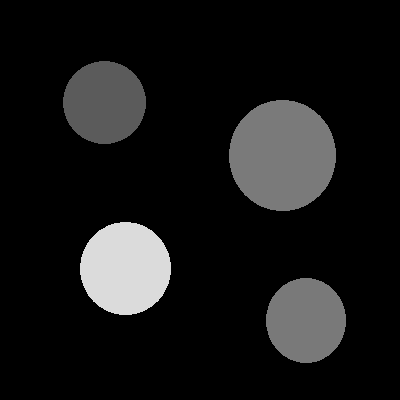
\includegraphics[width=\textwidth]{circulos4_1_original.png}
  \caption*{\footnotesize original}
\end{subfigure}
\begin{subfigure}[b]{0.19\textwidth}
  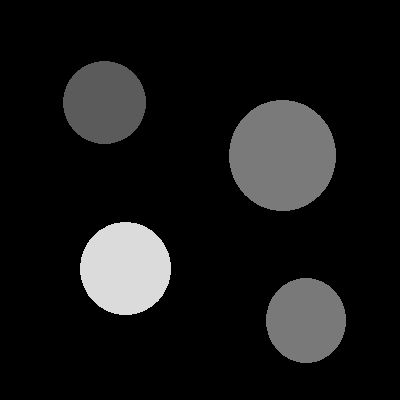
\includegraphics[width=\textwidth]{circulos4_2_filtrada.png}
  \caption*{\footnotesize filtrada}
\end{subfigure}
\begin{subfigure}[b]{0.19\textwidth}
  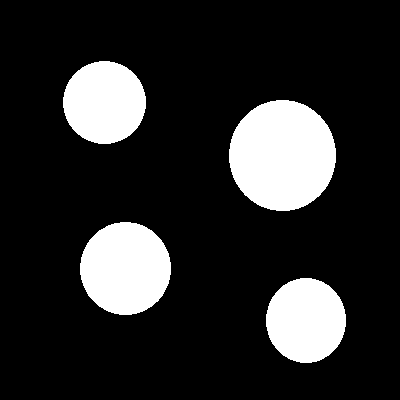
\includegraphics[width=\textwidth]{circulos4_3_binaria.png}
  \caption*{\footnotesize binária}
\end{subfigure}
\begin{subfigure}[b]{0.19\textwidth}
  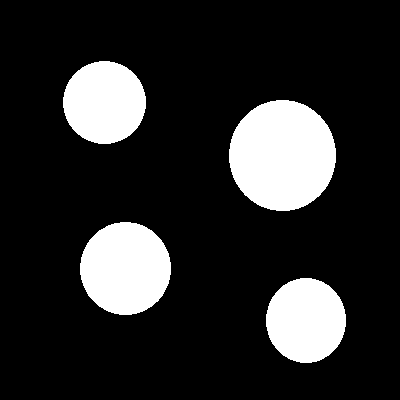
\includegraphics[width=\textwidth]{circulos4_4_morfologia.png}
  \caption*{\footnotesize morfologia}
\end{subfigure}
\begin{subfigure}[b]{0.19\textwidth}
  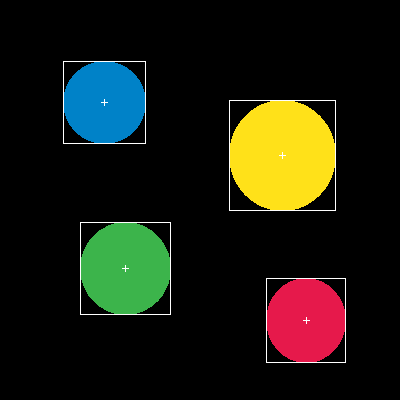
\includegraphics[width=\textwidth]{circulos4_5_rotulada.png}
  \caption*{\footnotesize rotulada}
\end{subfigure}
\caption{Etapas do processamento de \texttt{Circulos4.bmp}.}
\end{figure}

\begin{table}[H]
\centering
\begin{tabular}{rrrlrr}
\toprule
\textbf{Objeto} & \textbf{Área} & \textbf{Centroide} & \textbf{Bounding box} & \textbf{Perím.} & \textbf{Circ.} \\
\midrule
1 & 5329 & (306, 79)  & (266,37)--(345,121)  & 230 & 1,266 \\
2 & 6621 & (125, 131) & (80,85)--(170,177)   & 257 & 1,260 \\
3 & 9320 & (282, 244) & (229,189)--(335,299) & 307 & 1,243 \\
4 & 5391 & (104, 297) & (63,256)--(145,338)  & 232 & 1,259 \\
\bottomrule
\end{tabular}
\caption{Objetos identificados em \texttt{Circulos4.bmp}.}
\end{table}

Os quatro objetos foram identificados corretamente. As circularidades são
praticamente idênticas entre si, como esperado de quatro círculos, e as áreas
diferem porque os raios são diferentes.

% ---------------------------------------------------------------
\subsection{Imagem 2 --- com ruído (\texttt{Circulos4-ruido5.bmp})}

A mesma imagem anterior contaminada com ruído sal-e-pimenta em 5\% dos pixels,
gerada pelo próprio programa. Gerar a imagem por código, em vez de procurar
uma pronta, permitiu controlar a intensidade do ruído e dispor da imagem limpa
correspondente para comparação. Limiar de Otsu: $T = 0$.

\begin{figure}[H]
\centering
\begin{subfigure}[b]{0.19\textwidth}
  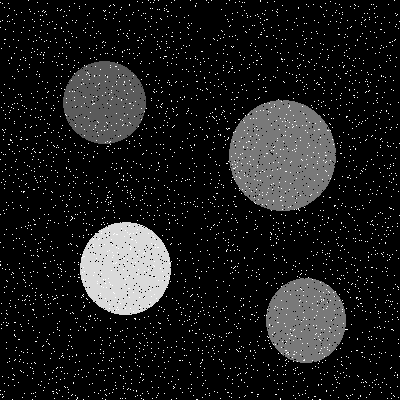
\includegraphics[width=\textwidth]{circulos4_ruido5_1_original.png}
  \caption*{\footnotesize original}
\end{subfigure}
\begin{subfigure}[b]{0.19\textwidth}
  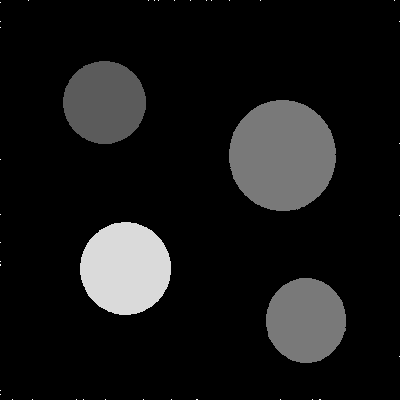
\includegraphics[width=\textwidth]{circulos4_ruido5_2_filtrada.png}
  \caption*{\footnotesize filtrada}
\end{subfigure}
\begin{subfigure}[b]{0.19\textwidth}
  
\includegraphics[width=\textwidth]{circulos4_ruido5_3_binaria.png}
  \caption*{\footnotesize binária}
\end{subfigure}
\begin{subfigure}[b]{0.19\textwidth}
  
\includegraphics[width=\textwidth]{circulos4_ruido5_4_morfologia.png}
  \caption*{\footnotesize morfologia}
\end{subfigure}
\begin{subfigure}[b]{0.19\textwidth}
  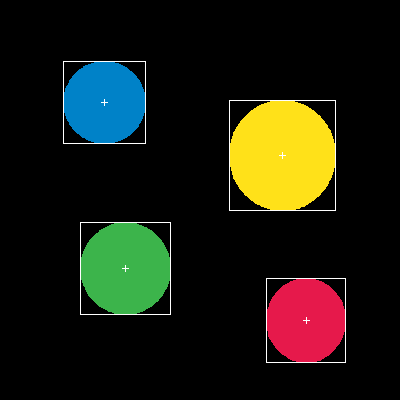
\includegraphics[width=\textwidth]{circulos4_ruido5_5_rotulada.png}
  \caption*{\footnotesize rotulada}
\end{subfigure}
\caption{Etapas do processamento de \texttt{Circulos4-ruido5.bmp}. A diferença
entre a primeira e a segunda imagem mostra a ação do filtro de mediana.}
\end{figure}

\begin{table}[H]
\centering
\begin{tabular}{rrrlrr}
\toprule
\textbf{Objeto} & \textbf{Área} & \textbf{Centroide} & \textbf{Bounding box} & \textbf{Perím.} & \textbf{Circ.} \\
\midrule
1 & 5335 & (306, 79)  & (266,37)--(345,121)  & 230 & 1,267 \\
2 & 6611 & (125, 131) & (80,85)--(170,177)   & 258 & 1,248 \\
3 & 9323 & (282, 244) & (229,189)--(335,299) & 307 & 1,243 \\
4 & 5390 & (104, 297) & (63,256)--(145,338)  & 233 & 1,248 \\
\bottomrule
\end{tabular}
\caption{Objetos identificados em \texttt{Circulos4-ruido5.bmp}.}
\end{table}

Comparando com a Imagem~1, as áreas diferem em no máximo 10 pixels
(0,15\%), os centroides são idênticos e as \emph{bounding boxes} coincidem.
O ruído foi integralmente absorvido pelo pré-processamento.

% ---------------------------------------------------------------
\subsection{Imagem 3 --- situação complexa (\texttt{C1.bmp})}

Imagem de $512 \times 384$ pixels com cinco figuras geométricas de tamanhos e
formas diferentes, escuras sobre fundo claro. Três são preenchidas e duas são
vazadas --- apenas o contorno. Limiar de Otsu: $T = 192$. Polaridade
detectada: objeto escuro.

\begin{figure}[H]
\centering
\begin{subfigure}[b]{0.19\textwidth}
  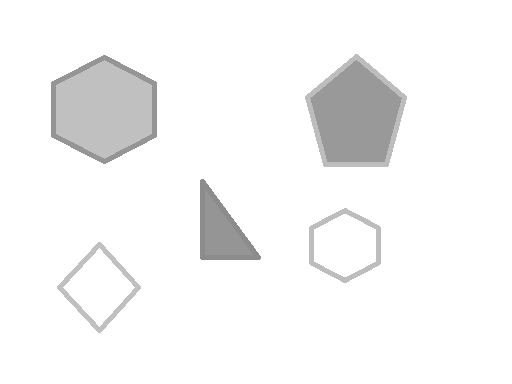
\includegraphics[width=\textwidth]{c1_1_original.png}
  \caption*{\footnotesize original}
\end{subfigure}
\begin{subfigure}[b]{0.19\textwidth}
  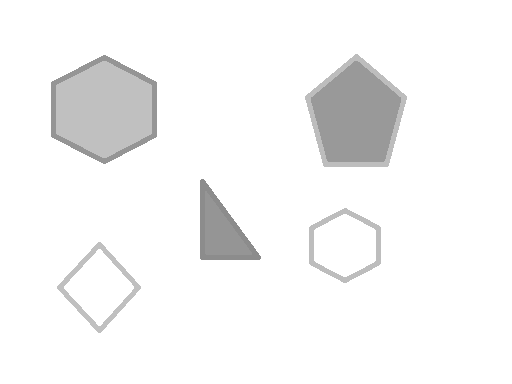
\includegraphics[width=\textwidth]{c1_2_filtrada.png}
  \caption*{\footnotesize filtrada}
\end{subfigure}
\begin{subfigure}[b]{0.19\textwidth}
  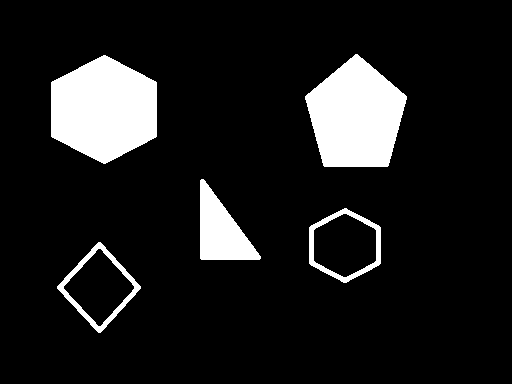
\includegraphics[width=\textwidth]{c1_3_binaria.png}
  \caption*{\footnotesize binária}
\end{subfigure}
\begin{subfigure}[b]{0.19\textwidth}
  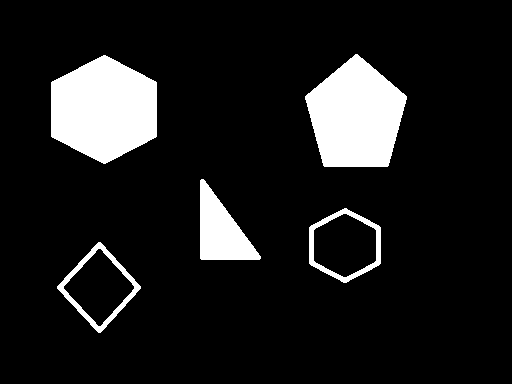
\includegraphics[width=\textwidth]{c1_4_morfologia.png}
  \caption*{\footnotesize morfologia}
\end{subfigure}
\begin{subfigure}[b]{0.19\textwidth}
  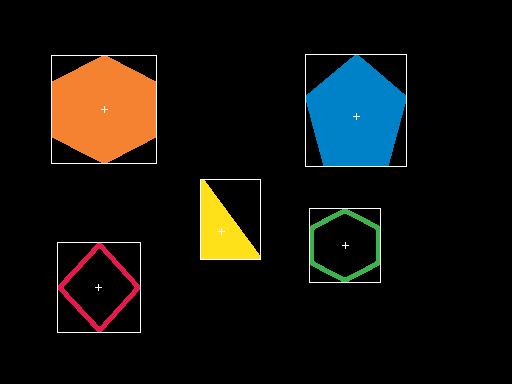
\includegraphics[width=\textwidth]{c1_5_rotulada.png}
  \caption*{\footnotesize rotulada}
\end{subfigure}
\caption{Etapas do processamento de \texttt{C1.bmp}.}
\end{figure}

\begin{table}[H]
\centering
\begin{tabular}{rrrlrr}
\toprule
\textbf{Objeto} & \textbf{Área} & \textbf{Centroide} & \textbf{Bounding box} & \textbf{Perím.} & \textbf{Circ.} \\
\midrule
1 & 1167 & (98, 96)   & (57,51)--(140,141)   & 344 & 0,124 \\
2 & 1106 & (345, 138) & (309,101)--(380,175) & 400 & 0,087 \\
3 & 2717 & (221, 152) & (200,124)--(260,204) & 220 & 0,705 \\
4 & 8114 & (356, 267) & (305,217)--(406,329) & 304 & 1,103 \\
5 & 8728 & (104, 274) & (51,220)--(156,328)  & 318 & 1,085 \\
\bottomrule
\end{tabular}
\caption{Objetos identificados em \texttt{C1.bmp}.}
\end{table}

Esta é a imagem mais informativa quanto à circularidade. Os objetos 4 e 5 são
figuras preenchidas e compactas, com $C > 1{,}0$. O objeto 3 é um triângulo
preenchido, forma menos compacta, com $C = 0{,}705$. Os objetos 1 e 2 são as
figuras \textbf{vazadas}: têm área pequena e perímetro enorme, porque o
contorno tem duas bordas --- externa e interna --- e a circularidade despenca
para 0,124 e 0,087. A medida separa com clareza três categorias de forma.

% ---------------------------------------------------------------
\subsection{Análise de histograma}

A Figura~\ref{fig:hist} compara os histogramas de duas imagens de naturezas
opostas e explica por que a limiarização funciona em uma e não na outra.

\begin{figure}[H]
\centering
\begin{subfigure}[b]{0.45\textwidth}
  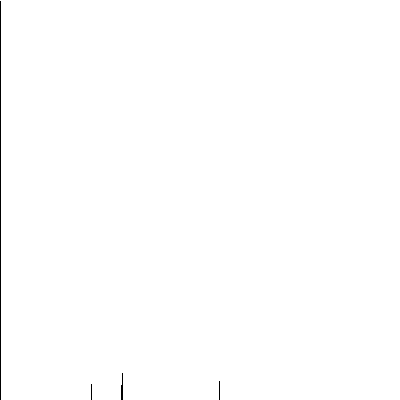
\includegraphics[width=\textwidth]{hist_circulos4.png}
  \caption{\texttt{Circulos4.bmp} --- picos isolados com vales largos entre eles.}
\end{subfigure}\hfill
\begin{subfigure}[b]{0.45\textwidth}
  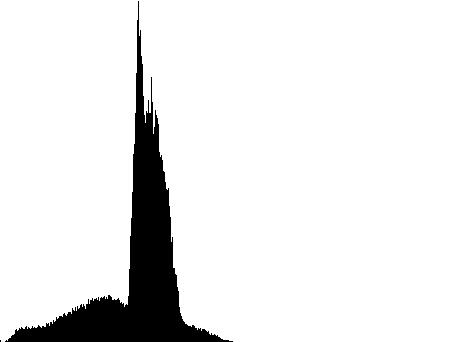
\includegraphics[width=\textwidth]{hist_abbey.png}
  \caption{\texttt{abbey.bmp} --- fotografia natural, distribuição contínua.}
\end{subfigure}
\caption{Histogramas de uma imagem sintética e de uma fotografia.}
\label{fig:hist}
\end{figure}

Em \texttt{Circulos4.bmp} os pixels se concentram em poucos níveis (0 para o
fundo, 122 e 218 para os objetos), separados por faixas vazias. Qualquer
limiar dentro de uma dessas faixas produz o mesmo resultado. Em
\texttt{abbey.bmp}, uma fotografia, o pico estreito corresponde ao céu --- uma
região extensa e quase uniforme --- e a base larga à alvenaria texturizada;
não existe vale, e nenhum limiar separa os dois.

% =====================================================================
\section{Discussão}
\label{sec:discussao}
% =====================================================================

\paragraph{O método conseguiu identificar todos os objetos?} Sim, nas três
imagens. Quatro objetos em \texttt{Circulos4.bmp}, quatro na versão ruidosa e
cinco em \texttt{C1.bmp}, todos conferindo com a contagem visual.

\paragraph{Houve falsos objetos?} Não no resultado final, mas houve em
abundância nas etapas intermediárias. A Tabela~\ref{tab:falsos} mostra a
contagem de componentes na imagem ruidosa conforme as etapas de limpeza são
ativadas.

\begin{table}[H]
\centering
\begin{tabular}{lr}
\toprule
\textbf{Configuração} & \textbf{Componentes} \\
\midrule
Sem mediana, sem morfologia, sem filtro de área & 2975 \\
Sem mediana, com morfologia, sem filtro de área & 40 \\
Com mediana, sem morfologia, sem filtro de área & 40 \\
Com mediana, com morfologia, sem filtro de área & 40 \\
\textbf{Com mediana, com morfologia, área $\geq$ 50 px} & \textbf{4} \\
\bottomrule
\end{tabular}
\caption{Componentes detectados em \texttt{Circulos4-ruido5.bmp} conforme as
etapas de limpeza. O valor correto é 4.}
\label{tab:falsos}
\end{table}

Sem nenhum pré-processamento, o sistema encontraria 2975 objetos onde existem
4: quase todo pixel de ruído isolado vira um componente. Vale notar que
mediana e morfologia são \emph{alternativas} nesta imagem --- cada uma sozinha
reduz de 2975 para 40 --- e que o filtro de área é o que fecha a conta.

\paragraph{Algum objeto foi perdido?} Nenhum. A comparação entre as
Tabelas de \texttt{Circulos4.bmp} e de sua versão ruidosa mostra que nem
mesmo as medidas foram afetadas de forma significativa: a maior diferença de
área é de 10 pixels em 6621, ou 0,15\%.

\paragraph{A escolha do limiar foi adequada?} Sim, e o histograma explica por
quê. Em \texttt{Circulos4.bmp} existe uma faixa larga de limiares que produzem
o mesmo resultado --- qualquer valor entre 1 e 121 separa igualmente bem, pois
não há pixel algum nessa faixa. O método de Otsu não precisou ser preciso,
apenas cair dentro do vale. Em \texttt{C1.bmp}, com $T = 192$, o resultado
também foi correto.

A robustez, porém, é propriedade da imagem, não do método. Testamos o mesmo
pipeline em \texttt{abbey.bmp}, uma fotografia, e nenhum limiar separa a
edificação do céu, porque o histograma não tem vale (Figura~\ref{fig:hist}).
A limiarização global pressupõe o fundo contrastante que o enunciado
estabelece.

\paragraph{A morfologia melhorou o resultado?} Sim, e de forma mensurável: na
Tabela~\ref{tab:falsos}, sozinha ela reduz a contagem de 2975 para 40.

Mais interessante é o \emph{tipo} de morfologia. Comparamos a abertura com a
erosão pura sobre a mesma imagem binária: a erosão remove o ruído, mas
continua consumindo os objetos a cada aplicação --- medimos um quadrado de 400
pixels caindo para 315 após uma erosão e para 231 após duas. A abertura remove
o mesmo ruído e devolve o tamanho: 399 pixels após uma aplicação, e 399
novamente após a segunda, isto é, a operação é idempotente. É essa propriedade
que a torna segura no pipeline.

\paragraph{O ruído afetou a identificação?} Não no resultado final, mas
afetaria drasticamente sem pré-processamento, como mostra a
Tabela~\ref{tab:falsos}. Quanto à escolha do filtro, medimos a diferença entre
média e mediana sobre uma imagem sintética com 5\% de ruído: a mediana
reconstrói a imagem original com erro médio de 0,05 níveis de cinza, contra
6,90 da média --- 138 vezes maior. O perfil atravessando uma aresta mostra a
razão:

\begin{table}[H]
\centering
\begin{tabular}{lrrrrrrr}
\toprule
\textbf{Coluna} & 37 & 38 & 39 & 40 & 41 & 42 & 43 \\
\midrule
Original & 40 & 40 & 40 & 200 & 200 & 200 & 200 \\
Mediana  & 40 & 40 & 40 & 200 & 200 & 200 & 200 \\
Média    & 40 & 40 & 93 & 146 & 200 & 200 & 200 \\
\bottomrule
\end{tabular}
\caption{Perfil de intensidade atravessando a borda de um quadrado. A mediana
preserva o degrau; a média o transforma em rampa.}
\end{table}

A média não remove o ruído impulsivo, ela o \emph{espalha}: um pixel branco
isolado vira uma mancha $3\times3$. A mediana o descarta e ainda preserva a
borda intacta. Por isso a mediana foi adotada no pipeline.

\paragraph{Quais limitações foram observadas?}

\begin{enumerate}
  \item \textbf{A morfologia não limpa a borda da imagem.} Como o elemento
    estruturante $3\times3$ não cabe sobre os pixels da moldura, esses pixels
    são preservados sem modificação. Verificamos que, dos 36 fragmentos de
    ruído que sobrevivem à abertura em \texttt{Circulos4-ruido5.bmp},
    \textbf{todos os 36 estão encostados na borda} e nenhum no interior. O
    filtro de área remove esses restos, mas a limitação existe.

  \item \textbf{O perímetro é subestimado, e a circularidade sai acima de
    1.} Contar pixels de contorno subestima o comprimento real, porque em um
    trecho diagonal cada pixel avança $\sqrt{2}$ mas conta como~1. Medimos a
    razão em círculos digitais de três raios diferentes (10, 20 e 40): o
    perímetro contado é sempre $0{,}891$ do valor teórico $2\pi r$. Como $P$
    entra ao quadrado no denominador da Equação~\ref{eq:circ}, a circularidade
    de um círculo sai em torno de 1,26 em vez de 1,0. Isso não invalida a
    medida --- a ordem entre as formas se mantém, que é o uso pedido --- mas o
    valor absoluto não deve ser lido como se 1,0 fosse o círculo perfeito.

  \item \textbf{A limiarização é global.} Um único limiar para a imagem
    inteira não lida com iluminação não uniforme. Limiarização adaptativa
    resolveria, ao custo de complexidade.

  \item \textbf{Objetos encostados são contados como um só.} A rotulação não
    tem como separar dois objetos que se tocam; seriam necessárias técnicas
    como a transformada de distância seguida de \emph{watershed}.

  \item \textbf{A detecção de polaridade pressupõe objetos minoritários.} Se
    os objetos ocupassem mais da metade da imagem, a heurística inverteria a
    classificação. O sistema permite sobrepor a decisão manualmente.
\end{enumerate}

% =====================================================================
\section{Conclusão}
% =====================================================================

O sistema atingiu o objetivo proposto: identificou corretamente todos os
objetos nas três imagens de teste, incluindo a versão contaminada com ruído, e
calculou cinco características geométricas para cada um deles. O trabalho
mostrou que a combinação de algoritmos simples --- contagem de pixels,
comparação com limiar, operações lógicas sobre vizinhança e busca em largura
--- resolve um problema de análise que nenhum deles resolveria isoladamente.

A lição mais clara dos experimentos é que \textbf{o pré-processamento não é
acessório}. A diferença entre 2975 falsos objetos e os 4 corretos não está no
algoritmo de rotulação, que é o mesmo nos dois casos, mas nas etapas de
limpeza que o antecedem. Do mesmo modo, a escolha entre média e mediana, que
parece um detalhe, define se as bordas dos objetos sobrevivem ao
pré-processamento.

A segunda lição é que a qualidade do resultado depende tanto da imagem quanto
do método. A limiarização global funcionou porque as imagens de teste têm
histograma com vales largos; na fotografia testada, nenhum limiar funciona.
Reconhecer essa dependência é parte de aplicar a técnica corretamente.

\paragraph{Possíveis melhorias.}

\begin{itemize}
  \item \textbf{Limiarização adaptativa}, calculando um limiar por região,
        para tolerar iluminação não uniforme;
  \item \textbf{Perímetro por rastreamento de contorno}, contabilizando
        $\sqrt{2}$ nos passos diagonais, o que corrigiria a escala da
        circularidade;
  \item \textbf{Separação de objetos encostados} por transformada de
        distância e \emph{watershed};
  \item \textbf{Tratamento das bordas} na morfologia, replicando os pixels da
        moldura em vez de preservá-los;
  \item \textbf{Descritores adicionais} --- excentricidade, momentos de Hu,
        número de Euler --- que permitiriam classificar os objetos por forma,
        e não apenas medi-los.
\end{itemize}

% =====================================================================
\section*{Referências}
\addcontentsline{toc}{section}{Referências}
% =====================================================================

\begin{thebibliography}{9}

\bibitem{gonzalez}
GONZALEZ, R. C.; WOODS, R. E.
\textbf{Processamento de Imagens Digitais}.
São Paulo: Edgard Blücher, 2000.

\bibitem{conci}
CONCI, A.; AZEVEDO, E.
\textbf{Computação Gráfica}. Volumes 1 e 2.
Rio de Janeiro: Campus, 2007.

\bibitem{otsu}
OTSU, N.
A Threshold Selection Method from Gray-Level Histograms.
\textbf{IEEE Transactions on Systems, Man, and Cybernetics},
v.~9, n.~1, p.~62--66, 1979.

\bibitem{aulas}
FURLAN, D.
\textbf{Notas de aula --- Processamento de Imagens}.
Universidade Tuiuti do Paraná, 2026.

\end{thebibliography}

\end{document}
